%! TEX program = pdflatex
\documentclass[]{hdsr}
%Graphics should all go in the figs/ directory
\graphicspath{{figs/}}

\begin{document}

% Larger bottom margin for the first page
\newgeometry{bottom=1.5in}

% Editorial staff will replace the following values:
% 1. Volume number
% 2. Issue number
% 3. Article DOI
% e.g. for Volume 2, Issue 3, DOI 12.345:
% \volumeheader{2}{3}{12.345}
%\volumeheader{0}{0}{00.000}



\begin{center}

  \title{The path to frictionless reproducibility is still under construction}
  \maketitle

  % Start page numbering on second page. Must appear *after* \maketitle
  \thispagestyle{empty}
  
  \vspace*{.2in}

  % Authors and Affiliations
  \begin{tabular}{cc}
    Lorena A. Barba\upstairs{\affilone,*},
   \\[0.25ex]
   {\small \upstairs{\affilone} The George Washington University} \\
  \end{tabular}
  
  % Replace with corresponding author email address
  \emails{
    \upstairs{*}labarba@gwu.edu 
    }
  \vspace*{0.4in}

%\begin{abstract}
%The abstract should be no more than 250 words.
%\end{abstract}
\end{center}

\vspace*{0.15in}
\hspace{10pt}
  \small	
  \textbf{\textit{Keywords: }} {reproducibility, open science, open data, open-source software}
  
\copyrightnotice

\section*{Media Summary}

It is said that science is advancing more rapidly than ever, due to the adherence to open sharing of data, code, methods and results. This may be true in some fields, but the reality is that the broad scientific community is still far from achieving frictionless reproducibility. I have many points of agreement with the article "Data Science at the Singularity" by David Donoho, but the scientific community needs to work harder to achieve the exemplars presented there. Challenges and opportunities in the pursuit of this ideal have to do with alignment of incentives, the need for better tools and platforms, training, and an unfinished cultural shift in the scholarly community.

\vspace{1cm}

\section*{Discussion of the Article "Data Science at the Singularity" by David Donoho}
\label{intro}
David Donoho's perspective paper ``Data Science at the Singularity'' argues that a transformative shift has occurred in computational research towards what he terms \emph{frictionless reproducibility} \citep{donoho2024data}. He says that the last decade has seen a remarkable acceleration in research progress in some fields, propelled by the maturation of three core data science principles: data sharing, code sharing, and competitive challenges, now implemented as frictionless open services. This new era of research is exemplified by the rapid advancements in empirical machine learning, which leverages frictionless reproducibility to markedly increase the pace of discovery and the spread of ideas. Donoho suggests that adhering to these principles allows for a seamless, efficient exchange of research outputs, fostering a community where innovation thrives on collective engagement and the iterative improvement of ideas.


% These commands need to appear at the point where you want
% the first page to end.
\restoregeometry
\newgeometry{bottom=0.5in}



In the field of machine learning the practices of open sharing of data and code, and competitive challenges have become the standard at various conferences and publication venues.
Many journals and top conferences, like NeurIPS (Neural Information Processing Systems), ICML (International Conference of Machine Learning), and ICLR (International Conference on Learning Representations), encourage or require authors to submit code and data along with their papers. 
ICML 2019 was the first time in a major machine learning conference when authors were encouraged to submit code along with their manuscripts, and reviewers were encouraged to consider the code in their review \citep{chaudhuri2019}.
The organizers reported that  36\% of more than 3000 submissions included code, and 67\% of the 774 accepted papers did so (noting that the acceptance rate for papers with code was slightly higher).
NeurIPS 2019 also for the first time experimented with a voluntary code submission policy (for accepted papers), as well as creating a new role of Reproducibility Chair \citep{pineau2019neurips}. A later report on the experiment noted that 40\% of 6743 submitted papers included code, and 74.4\% of accepted papers did so \citep{pineau2021improving}.
Also in 2019, the journal \emph{Nature Machine Intelligence} introduced a policy that when code is central to the results presented in the paper, the code must be made available to readers \citep{editorial2019naturemi}. The policy requires authors to include a Code Availability statement in the paper, describing how the code can be accessed and any applicable restrictions.
Today, the NeurIPS code submission policy is still voluntary,\footnote{\url{https://web.archive.org/web/20240303205540/https://neurips.cc/public/guides/CodeSubmissionPolicy}} but the conference has published a set of best practices for sharing code, including a completeness checklist.\footnote{\url{https://github.com/paperswithcode/releasing-research-code}}
ICML author guidelines state that ``easy availability of code will be taken into account in the decision-making process'' while still being optional.\footnote{\url{https://icml.cc/Conferences/2024/AuthorInstructions}}

Other scientific communities are similarly placing increasing importance on data and code sharing. On the same year that NeurIPS introduced the new role of Reproducibility Chair (2019), I held that same position in the committee of The International Conference on High-Performance Computing, Networking, Storage and Analysis, informally known as the Supercomputing conference, or SC.\footnote{\url{https://sc19.supercomputing.org/submit/reproducibility-initiative/}} We made it mandatory for all papers submitted to the SC19 Technical Program to include an appendix describing any digital artifacts associated with the research \citep{barba2021trustworthy}. The artifacts could be code, data, or other digital objects, and the appendix had to include a statement about the availability of these artifacts. 
Artifact Description appendices were independently reviewed in an innovative double-open peer-review process (while the paper underwent double-blind review). Reviewers checked on the availability of the artifacts and determined eligibility for one of the three levels of recognition badges: artifacts available, artifacts evaluated, and results validated.\footnote{ACM Artifact Review and Badging Version 1.1 - August 24, 2020. \url{https://www.acm.org/publications/policies/artifact-review-and-badging-current}}
The SC Reproducibility Initiative is one of the early examples of a major computing conference in a field outside of machine learning developing policies to encourage and recognize reproducibility and open science practices. A survey of the community in 2020 showed that 90\% of respondents were aware of issues related to reproducibility in computational and computer science, and overall the initiative has had a positive impact on the quality of the science published at the conference \citep{plale2021reproducibility}.
An inspection of the allocation reports of major computing resources in the US at the time, however, showed that hardly any of the projects awarded time on these supercomputers made code and data available \citep{barba2021trustworthy}.
Today,\footnote{March 4, 2023} a filter search in the ACM Digital Library for papers published in the past 5 years with an Artifacts Available badge returns 3,611 results, out of 726,224 records, or 0.5\% of the total; see Figure~\ref{fig:acm_badges_5years}.
This is a clear indication that the cultural shift towards open science practices is still in progress, and that the community needs to work harder to achieve the exemplars presented in Donoho's article.
And even when a compute-intensive research project is purposely open in its practices, such as the LIGO collaboration that led to the 2016 discovery of gravitational waves, authors report facing challenges in reproduction efforts, despite the availability of data and code supplementing the original publication \citep{brown2021reproducing}. The LIGO collaboration founded and curates the Gravitational Wave Open Science Center,\footnote{\url{http://gw-openscience.org}} which hosts data, software, documents and other tools for the community and public. Yet, when Brown et al.\ exercised the open data and code to reproduce the analysis of the signal detection, they came across omitted code versions and figure scripts in the research compendium. The challenges in reproducing the results of the LIGO discovery are a reminder that the ideal of frictionless reproducibility is still far from being achieved.

\begin{figure}
    \centering
    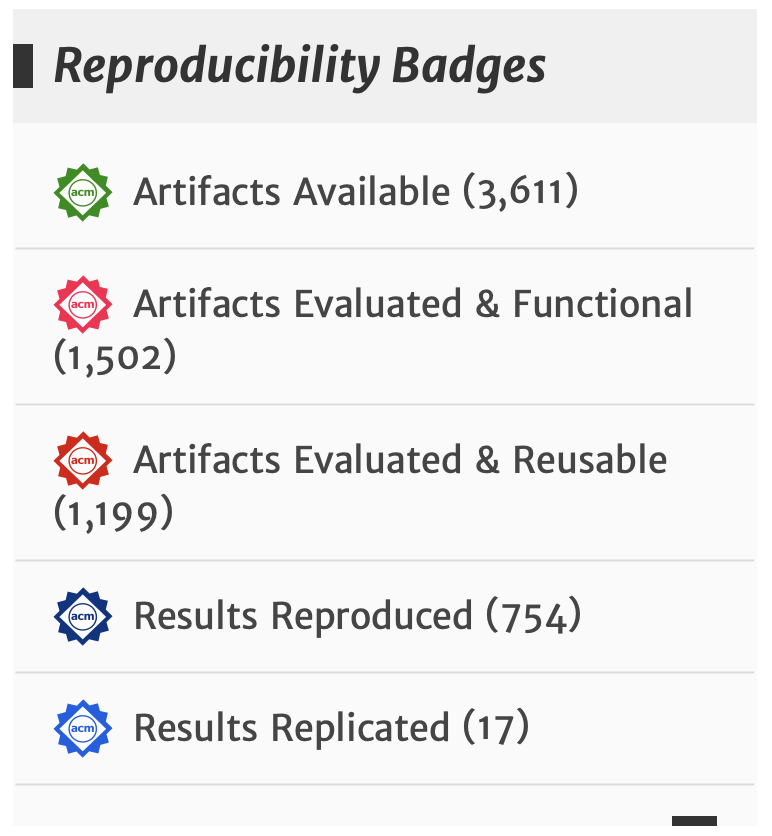
\includegraphics[scale=0.4]{acm_badges_5years-a} \\
    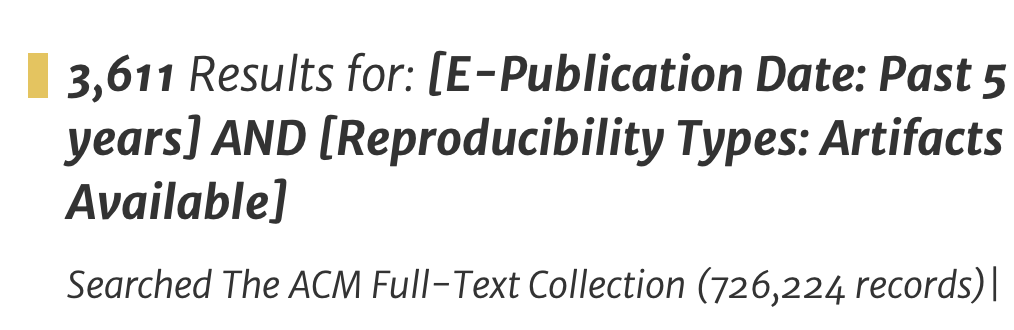
\includegraphics[scale=0.45]{acm_badges_5years-b} \\
    \caption{Results from a filter search in the ACM Digital Library for papers published in the past 5 years with an Artifacts Available badge.}
    \label{fig:acm_badges_5years}
\end{figure}

The mature principle of data sharing, exemplified by open access to datasets across various disciplines, has certainly had enormous impact. This practice allows researchers to readily access, analyze, and build upon existing data, enhancing the reproducibility of research findings and fostering a culture of collaboration.
The impact of such a culture of research data sharing is epitomized by the story of the Protein Data Bank (PDB), now an essential repository for structural data of biological molecules. Established in 1971, the PDB evolved over the years to become a global resource, freely accessible to the scientific community, which transformed the field of molecular biology. From its initial 7 molecular structures, the PDB reached a milestone of 200,000 entries in 2019,\footnote{\url{https://www.rcsb.org/news/639b9e337f8444f313d20414}} data that is used by researchers worldwide to understand the structure and function of biological macromolecules. Such scale enabled the application of machine learning techniques for protein-structure prediction, culminating in the success of DeepMind's AlphaFold algorithm, which won the Critical Assessment of Structure Prediction (CASP) competition in 2018 and 2020 \citep{jumper2021highly}. The PDB is a testament to the transformative power of open data sharing, and its success has inspired the creation of similar repositories across various scientific domains.

The field of machine learning has its own stories of data-sharing success, one of the most famous of which is probably ImageNet. Founded by Professor Fei-Fei Li, the ImageNet database went from zero to three million categorized images in 2008, and reached more than 11 million images by mid-2010. That year saw the first ImageNet Large Scale Visual Recognition Challenge (ILSVRC), in which teams competed to programmatically categorize a subset of the images in the database. The competition, held annually until 2017, was a catalyst for the development of deep learning techniques.\footnote{\url{https://image-net.org/challenges/LSVRC/}} Like in the case of the PDB and the CASP challenge, ImageNet and the ILSVRC serve as example of the combined power of open data sharing and competitive challenges to drive innovation and discovery, as Donoho describes.

David Donoho proposes that the synergistic combination of open data sharing, code sharing, and the organization of competitive challenges leads to unprecedented acceleration of computational research. When the global research community mobilizes to participate in competitions around shared datasets and agreed-upon benchmarks, the resulting collective engagement and iterative improvement of ideas leads to rapid progress: frictionless, and reproducible. He says this brings ``a drop to zero of the human effort required to reproduce a computational result.'' Let's see how this might be consummated.

For Donoho's model of frictionless reproducibility to be practicable, several underlying tools and skills are presumed to exist within the community. These include:

\begin{enumerate}
    \item Data repositories and data-sharing platforms---these are essential for the storage, curation, and dissemination of research data. They should be designed to facilitate easy access, search, and retrieval of data, and should implement the FAIR principles (Findable, Accessible, Interoperable, Reusable) \citep{wilkinson2016fair}.
    \item Code sharing and execution environments---these are platforms that allow researchers to share the code and the environment in which it was executed, and to execute code in a reproducible manner. They should capture the computational environment, including the software stack, libraries, and dependencies, and enable the sharing of the entire computational environment along with the code.
    \item Virtualization and containerization technologies---these allow researchers to package their code and computational environment into a single, portable container that can be executed on any platform. They ensure that computational experiments can be re-executed in consistent environments, addressing the challenge of so-called ``dependency hell'' and environment reproducibility.
    \item Collaborative development skills---these are key for developing shared code and contributing to data repositories. They include skills in version control, collaborative coding, and the use of collaborative platforms like GitHub, GitLab, or Bitbucket.
    \item Data-management skills---these are required for curating, annotating, and sharing research data. They include skills in data management planning, metadata creation, data curation and understanding of archival practices including the use of global persistent identifiers.
\end{enumerate}

David Donoho's vision is compelling and merits broad support. I too want to be part of a future where scientific discovery is not just rapid but also transparent, reproducible, and accessible to a global community of researchers. However, the current state of affairs reveals significant gaps in both scholarly infrastructure and human capital that hinder the full realization of Donoho's model of frictionless reproducibility. While there has been progress in developing data repositories and code-sharing platforms, we face inconsistent standards, limited interoperability, and varying levels of sustainability of these resources. A lack of unified protocols and support can make it challenging for researchers to share and access data and code effectively. Moreover, while virtualization and containerization technologies have made strides, their adoption is far from universal, and many researchers face technical barriers to implementing these solutions. Finally, the skills needed for participating in this new ecosystem are not uniformly distributed across the research community. Collaborative development skills, data management proficiency, and the ability to navigate virtualization technologies are highly specialized and not typically part of traditional academic training. This creates a divide between those who can engage in these practices and those who cannot, potentially exacerbating disparities in research output and impact.

The diffusion of Donoho's model relies on a skilled workforce adept in data management, software development, and collaborative research practices. But our current education and training programs are not equipping researchers with these interdisciplinary skills. Expanding training programs and integrating these skills into the curriculum of scientific and engineering disciplines is critical.
Donoho acknowledges the lag in adapting educational programs to the demands of a data science and computationally literate workforce and the omissions in current academic curricula. An interdisciplinary approach to education is needed, bridging the gap between computational sciences, statistics, and domain-specific knowledge. We may need to incorporate practical, hands-on experience through projects, internships, and collaborations with industry and research institutions. We should emphasize the importance of open science practices, including data and code sharing, and the principles of reproducible research. This can be achieved through coursework that requires students to share their own work in a reproducible manner and to critically evaluate the reproducibility of existing research. Such elements are already being incorporated into the curriculum of some data science and computational science programs, but they are not yet widespread.

The current academic and research incentive structures, which prioritize novel findings and high-impact publications, does not adequately reward the time and effort spent on sharing data and code or on ensuring reproducibility. Revising incentive structures to recognize these contributions is necessary to foster a culture of open sharing and collaboration. This may involve recognizing data and code sharing as a scholarly output, and incorporating these contributions into hiring, promotion, and tenure decisions. It may also involve recognizing the value of reproducing and validating existing research, and rewarding researchers who engage in these activities. In my own experience, I have found that the recognition of open science practices in hiring and promotion decisions is still rare, and that the broader academic community is far from achieving the exemplars presented in Donoho's article.

\section*{Conclusion}
David Donoho's vision of frictionless reproducibility is a compelling model for the future of computational research. The principles of open data sharing, code sharing, and competitive challenges have already had a transformative impact on the field of machine learning, and have the potential to accelerate research progress across various scientific domains. However, the realization of this vision is contingent on the development of scholarly infrastructure and human capital that support these practices. We need to expand data repositories and code-sharing platforms, develop unified protocols and standards, and ensure the sustainability of these resources. We need to promote the adoption of virtualization and containerization technologies, and provide training and support to researchers who face technical barriers to implementing these solutions. Training programs are needed integrating interdisciplinary skills into the curriculum of scientific and engineering disciplines. Most of all, reform of academic and research incentive structures is needed to recognize the value of open science practices and reproducible research. Achieving these goals will require a concerted effort from the global research community, and the signs of change are not yet visible. The future of computational research is bright, but the path to frictionless reproducibility is still under construction.


% 1. When figure position is crucial, use the [H] tag 
%    to enforce absolute positioning
% 2. Image files should be referenced without file extension
%\begin{figure}[H]
%    \centering
%    \includegraphics[scale=0.35]{iris_pairs} \\
%    \caption{This is an example figure}
%    \label{fig:my_label}
%\end{figure}


\subsection*{Disclosure Statement}
The authors have no conflicts of interest to declare.

%\subsection*{Acknowledgments}

 
%\subsection*{Contributions}



%Begin appendix section(s)
%\appendix

% Add appendices here:
%\section{Title}
%\label{appendix-customize-this-label}






% All references should be stored in the file "references.bib"
% Please do not modify anything below this line.
\printbibliography



\end{document}